\chapter{Results}

[TODO: Discuss in general the graphs of $M$ in the contest of a phase transition?]

\section{1D Ising model}

The one dimensional Ising model is known not to present a phase transition at any finite temperature ($T_C > 0$).

\begin{figure}[htbp]
	\centering
	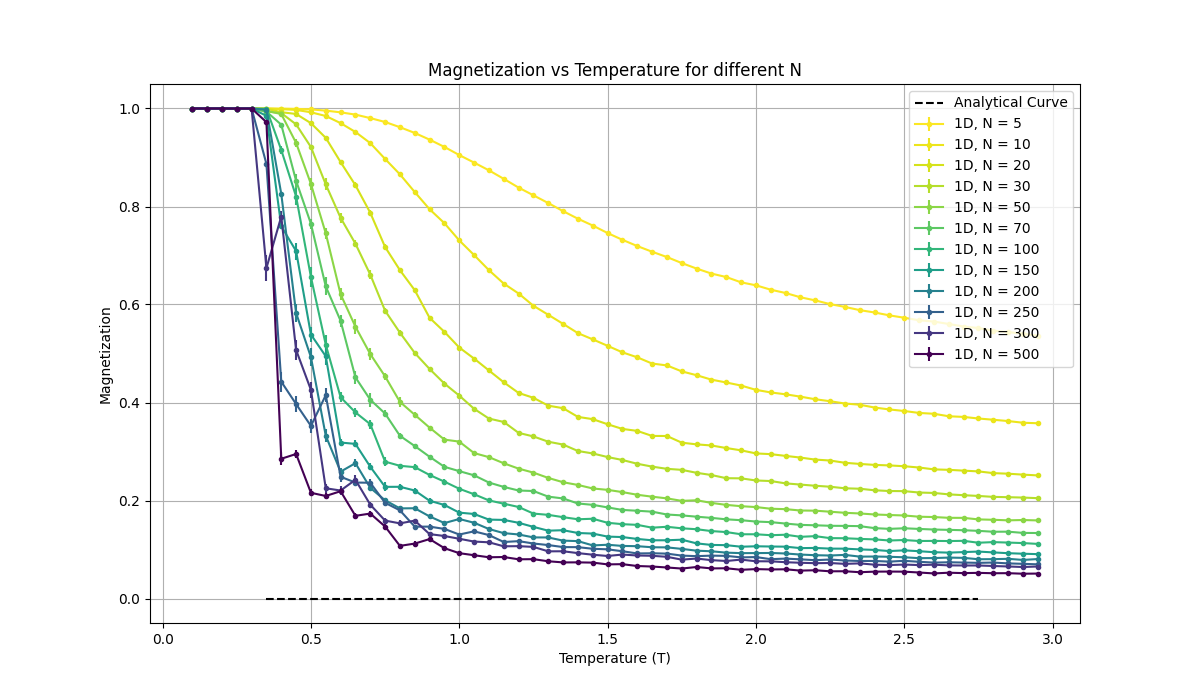
\includegraphics[width=1.\textwidth]{../pics_and_anims/magn_graphs/magnetization_convergence_1D.png}
	\caption{Magnetization for the 1D Ising model.}
	\label{fig:1D_magn}
\end{figure}

What can be seen in figure \ref{fig:1D_magn} is that the magnetization $M(T)$ approaches a constantly null function as $N$ increases. This is consistent with the theoretical prediction. The value close to $1$ are simply an effect of finite-size corrections: the critical temperature would be exactly $0$ with infinite size. The reason why increasing the size of the system leads to the movement of the "step" towards $0$ is that the energy cost of breaking a streak of aligned spins is independent of the size of the system, which means that for bigger $N$ the probability of having a single big streak of aligned spins is lower, and for every streak of aligned-up spins there is a high probability a streak of a same length of aligned-down spins to exist, which leads to a null magnetization. Since the flipping of a spin is an effect of thermal fluctuations the magnetization is closer to zero for higher temperatures (this can be seen in the curves of the smaller lattices: they don't drop instantly but smoothly curve towards zero), but this effect is negligible for bigger lattices, where the magnetization drops to zero faster.

\section{2D Ising model}

The two dimensional Ising model presents a nicer result, as it is known to present a phase transition at a finite temperature. This is directly translated in the approach to a step function of the magnetization $M(T)$ as $N$ increases, which can be seen in figure \ref{fig:2D_magn}.

\begin{figure}[htbp]
	\centering
	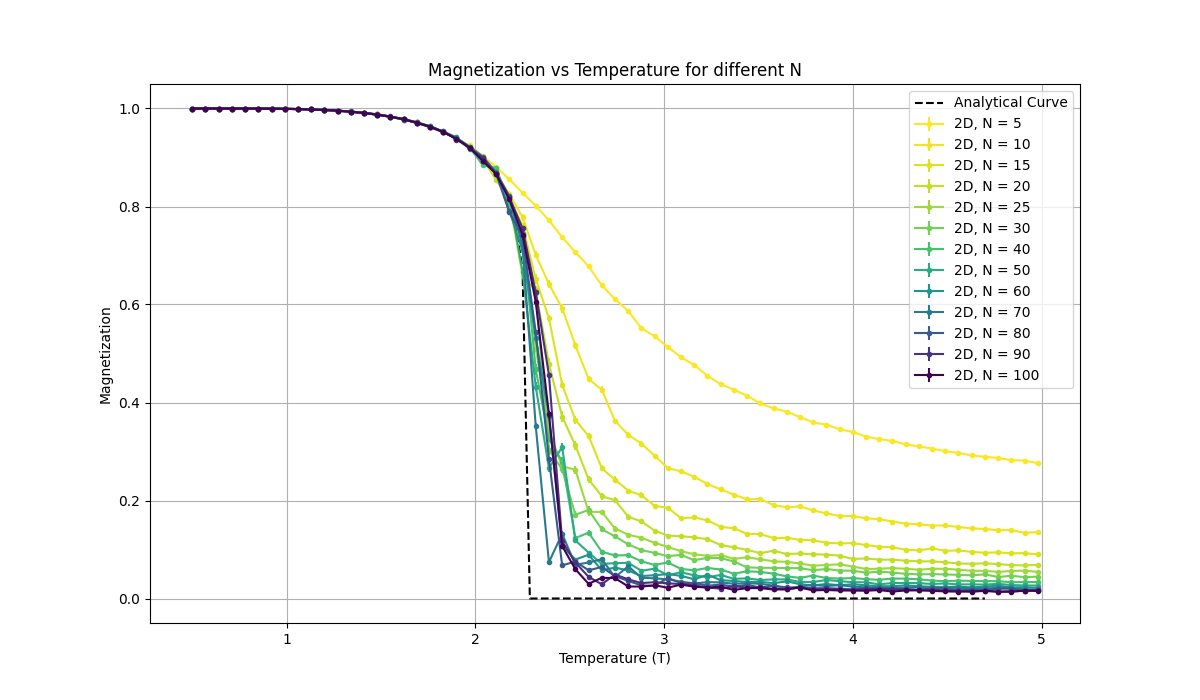
\includegraphics[width=1.\textwidth]{../pics_and_anims/magn_graphs/magnetization_convergence_2D.png}
	\caption{Convergence of magnetization for the 2D Ising model.}
	\label{fig:2D_magn}
\end{figure}

The accepted value for the critical temperature of the 2D Ising model is $T_C \approx 2.269$. [TODO: add extracted value of $T_C$]

The difference between the 1D and 2D Ising model is that in the 2D case a single spin flip is enough to break a streak of aligned spins, that is, the a single spin flip che change significantly the contribution to the magnetiziation of a section of the lattice. The equivalent of a streak of aligned spins in 2D is a cluster of aligned spins, and the equivalent of a single spin flip to break the streak is the flipping of the spins on the border of the cluster. The energy needed to flip a single spin is still independent of the size of the system, but the size of the perimeter of a cluster is not, and this introduces a size dependence in the probability of having a cluster of aligned spins, which is what leads to a threshold behavior.

\section{3D Ising model}

The same argument for the 2D Ising model can be applied to the 3D case, and the results are similar. The accepted value for the critical temperature of the 3D Ising model is $T_C \approx 4.5115$. [TODO: add extracted value of $T_C$]

\begin{figure}[htbp]
	\centering
	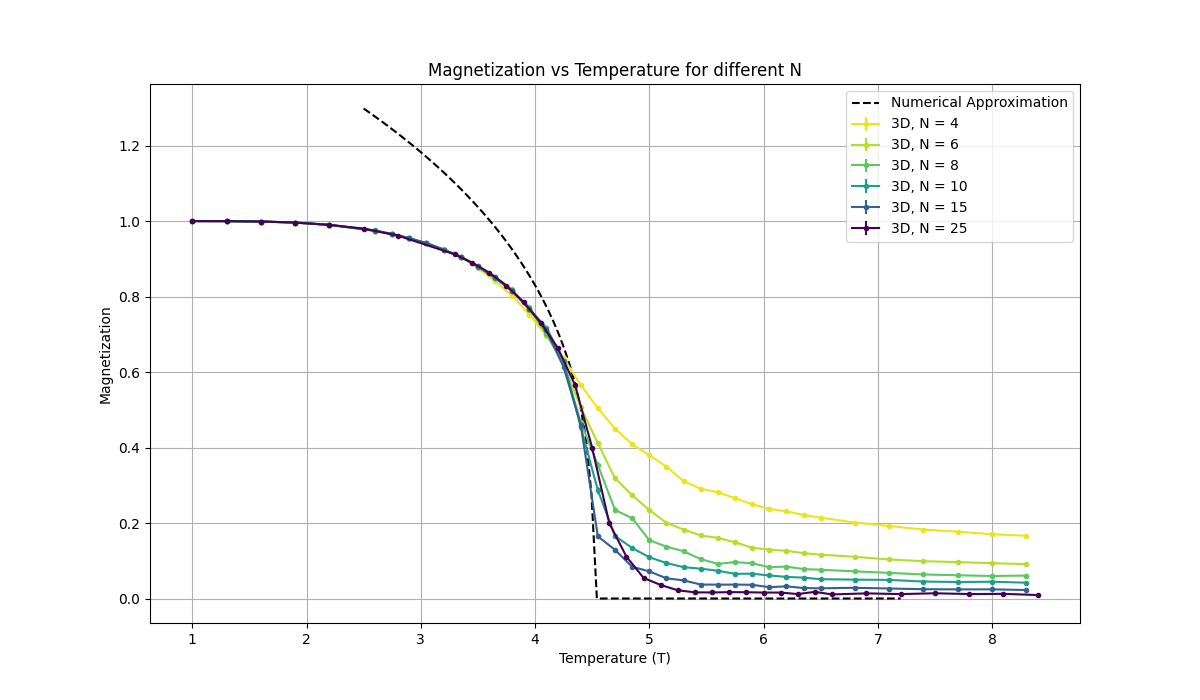
\includegraphics[width=1.\textwidth]{../pics_and_anims/magn_graphs/magnetization_convergence_3D.png}
	\caption{Convergence of magnetization for the 3D Ising model.}
	\label{fig:3D_magn}
\end{figure}

The theoretical difference is that the 3D model is not analytically solved (in the plot the numerical results are confronted with a critical scaling behavior [TODO: fonte maybe  A L Talapov and H W J Blöte 1996 J. Phys. A: Math. Gen. 29 5727]), but the existence of a phase transition is well-established, and the numerical results are consistent with the expected behavior.

\clearpage